\documentclass[final,10pt]{phdimt}





% list here the bibfiles you want to use
% note that you have to add the extension since the template uses
% biblatex and biber to compile the references
\addbibresource{references.bib}
\addbibresource{mainmatter/2/methods_and_methods.bib}

% LaTex metadata (used in the frontmatter)

\title{A Thesis to rule them All:\\An Agent Based approach}
\author{<author>}
\mail{<author>@imtlucca.it}
\phdname{PhD in Institutions, Markets and Technologies}
\curriculum{Economics, Management and Data Science}
\coordinator{<coordinator>}
\coordinatorinst{\IMT{}}
\cycle{XXXI}
\pubyear{2018}

%% Uncomment the following section if you want to set PDF Metadata
% \pdfinfo{
% 	/Title  ()
% 	/Creator (VSCode)
% 	/Producer (pdfTeX)
% 	/Author ()
% 	/Subject (Economics)
% 	/Keywords (mobility)
% }
% \pdfcatalog{
% 	/PageMode (/UseOutlines)
%       /OpenAction (fitbh)
% }


\supervisor{Prof.\ <supervisor>}
\supervisorinst{\IMT{}}
\cosupervisor{Prof.\ <co-supervisor>}
\cosupervisorinst{<co-supervisor institution>}
\tutor{<tutor>}
\tutorinst{<tutor institution>}

% Set revieweres here.
\firstreviewer{<Reviewer 1>}
\firstreviewerinst{<Reviewer 1 institution>}
\secondreviewer{<Reviewer 2>}
\secondreviewerinst{<Reviewer 2 institution>}
\thirdreviewer{}
\thirdreviewerinst{}

\begin{document}

% Let's do not cheat on line spacing
\renewcommand\baselinestretch{1}
\baselineskip=14pt


\frontmatter

\pagestyle{empty} % following pages do not require page numbering
\maketitle{}
\makereviewerspage{}
% !TEX root =  ../thesis.tex
\begin{dedication}

\end{dedication}
\pagestyle{plain} % numbering is shown from now on

\tableofcontents
\listoffigures
\listoftables
\begin{acknowledgements}
\addcontentsline{toc}{chapter}{Acknowledgements}

% Acknowledgments may be optional except in either of the following circumstances.
%
% 1. The student reproduces/reprints copyrighted material requiring permission
%    to be reprinted/reproduced in which case the student isresponsible for
%    acquiring and acknowledging each permission to reprint/reproduce.
% 2. The student uses as text in a chapter either material based on co-authored
%    published or about to be published articles or material based on co-authored
%    papers in progress.
%    The student should identify all co-authors, the journal where the article
%    can be found and the journal publisher.

\end{acknowledgements}

% !TEX root =  ../thesis.tex
% Don't modify the following
% Note that if the table is too long, it will flow out of the page. If you have a very long CV, maybe you're smart enough to solve this problem by yourself! :)
\begin{center}
\vspace*{0.5cm}
{\Large \bf  Vita}
\addcontentsline{toc}{chapter}{Vita and Publications}
\end{center}
\begin{table}[h!]
\begin{center}
\renewcommand{\arraystretch}{1.25}
\begin{tabular*}{1\textwidth}{l p{8.5cm}}

% Edit content of this part (just the content!)
{\bf Mach 14, 1879} & Born, Ulm (W\"urttemberg), Germany \\
& \\
{\bf 1900} & Degree in Physics\\
& Final mark: 110/110 cum laude\\
& ETH Z\"urich, Z\"urich, Switzerland \\
& \\
{\bf 1903} & Assistant Examiner\\
& Federal Office for Intellectual Property\\
& Bern, Switzerland \\

% Don't modify the following
\end{tabular*}
\end{center}
\end{table}
% Comment the following if you do not prefer the publications to start on a different page
\clearpage
\begin{center}
\vspace*{0.5cm}
{\Large \bf  Publications}
\end{center}
\vspace*{0.5cm}
{\small
\begin{enumerate}

% Edit content of this part (just the content!)

\item A.~Einstein, ``Conclusions Drawn from the Phenomena of Capillarity,'' in \emph{Annalen der Physik}, vol.~4, pp.~513, 1901.

\item A.~Einstein, ``On a Heuristic Viewpoint Concerning the Production and Transformation of Light,'' \emph{Annalen der Physik}, vol.~17, pp. 132 -- 148, 1905.

% Don't modify the following
\end{enumerate}
}
% Comment the following if you do not prefer the publications to start on a different page
\clearpage
\begin{center}
\vspace*{0.5cm}
{\Large \bf  Presentations}
\end{center}
\vspace*{0.5cm}
{\small
\begin{enumerate}

% Edit content of this part (just the content!)

\item A.~Einstein, ``On the Electrodynamics of Moving Bodies,'' at \emph{University of Z\"urich}, Z\"urich, Switzerland, 1905.

% Don't modify the following
\end{enumerate}
}
% !TEX root =  ../thesis.tex
\begin{abstract}
\addcontentsline{toc}{chapter}{Abstract}
% Max 1 page. The abstract consists of:

% - a brief statement of the problem;
% - a brief exposition of the method or procedures used;
% - a condensed summary of the findings of the study.
% The abstract is published without further editing or revisions and special care must be taken in its preparation.


\end{abstract}



\mainmatter{}

% !TEX root =  ../../thesis.tex
\graphicspath{{mainmatter/2/figures/}}


\chapter{Introduction}\label{chapt:introduction}


This is some text which will cite \citet{Einstein:1905:EBK}.
Note that the you can use \texttt{natbib} commands to mark up citations (i.e. \texttt{citet}, \texttt{citep}, \texttt{citeauthor})
Also, you can add a footnote with the "footnote" command. \footnote{This is a footnote.}
Footnote numbering is automatically managed.\footnote{This is the second footnote.}

% !TEX root = ../../thesis.tex

\graphicspath{{mainmatter/2/figures/}}

\chapter{Methods, Methods and more Methods}\label{ch:methods}

Here I will cite \citet{Torvik2009} a references saved in \texttt{mainmatter/2/methods\_and\_methods.bib} which has been loaded in the root file \texttt{thesis.tex}

\begin{figure}[htbp]
    \centering
    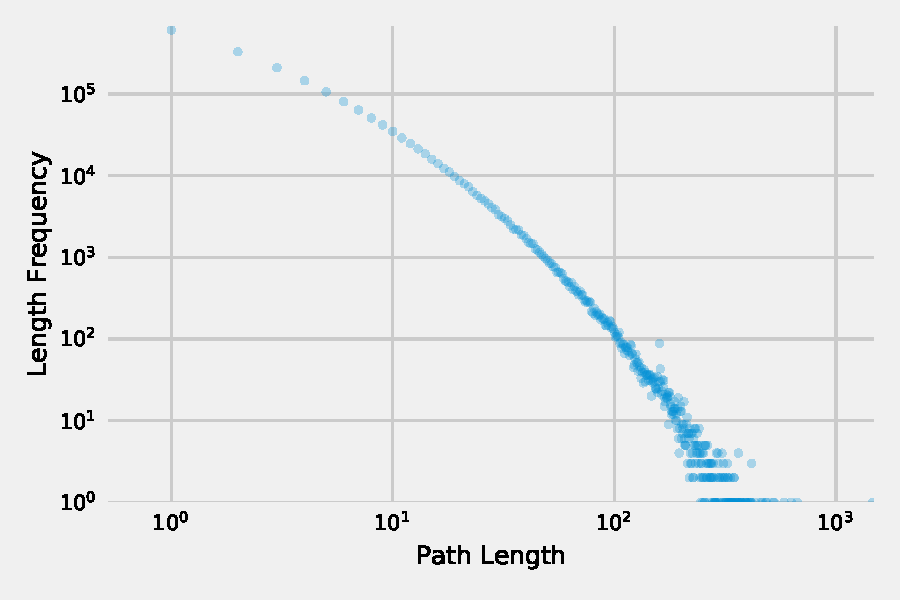
\includegraphics[width=0.95\textwidth]{mainmatter/2/figures/path_distribution.pdf}
    \caption{The distribution of career path lengths.}
    \label{fig:path_distribution}
\end{figure}


\chapter{Conclusion}\label{ch:conclusion}

\appendix
% !TEX root =  ../../thesis.tex

\chapter{Appendix Title}\label{app:nobel}




\printbibliography{}
\makecopyright{}

\end{document}
